% Chapter 3 (from main tex file)
% Research Project
% Author: Javier Reyes

\chapter{Embedded Linux} \label{embedded-linux}

In order to have a usable stack implementation of Ethernet communication, it is recommended to boot an OS in the device, considering time and complexity for a standalone driver implementation of an Ethernet stack driver for the specific hardware configuration present in the Zynqberry.

Xilinx provides a workflow to create an embedded Linux image fitted for the ARM architecture, by means of a provided tool (a collection of command-line programs) to configure and compile Linux-based images focused on Xilinx hardware, using Yocto Project.

\section{Xilinx Petalinux}

Xilinx Petalinux is an Embedded Linux System Development Kit for Xilinx FPGA-based System-on-Chip devices\cite{UG1144}. It is based on Yocto Project SDK's for the Xilinx hardware architectures (Zynq, Zynq UltraScale+, MicroBlaze full and lite).

The specific workflow for the tool can be different depending on the hardware platform and the desired application(s). As a reference, an overview flow is shown in the table \ref{table:design-flow-overview}.

\begin{table}[ht]
	\centering
	\footnotesize
	\begin{tabular} {| l | l |}
		\hline
		\textbf{Design Flow Step} & \textbf{Tool / Workflow} \\ [0.25cm]
		\arrayrulecolor[HTML]{B20738} 
		\hline \arrayrulecolor[HTML]{000000}
		Hardware Platform Creation & Vivado \\
		\hline
		Create Petalinux Project & petalinux-create -t Project \\
		\hline
		Initialize Petalinux Project & petalinux-config --get-hw-description \\
		\hline
		Configure System-Level Options & petalinux-config \\
		\hline
		Create User Components & petalinux-create -t COMPONENT \\
		\hline
		Configure the Linux Kernel & petalinux-config -c kernel \\
		\hline
		Configure the Root Filesystem & petalinux-config -c rootfs \\
		\hline
		Build the System & petalinux-build \\
		\hline
		Deploy the System & petalinux-package \\
		\hline
		Test the System & petalinux-boot \\
		\hline
	\end{tabular}
	\caption{Design Flow Overview, from \cite{UG1156}}\label{table:design-flow-overview}.
\end{table}

The Zynqberry board has a specific hasrdware configuration that requires a unique flow for building an embedded Linux image. Therefore, most of the standard flow cannot be applied directly. The followed procedure for this project is detailed in the Appendix \ref{appen1}.

\section{Yocto Project}

The core of the Petalinux tool is the Yocto SDK, an open-source community project that allows to create custom Linux-based systems for embedded products, independent of the hardware architecture. It consists of a flexible toolset and a development environment, allowing software customizations and build interchange for multiple hardware platforms as well as maintainable and scaled software stack.

\begin{figure}[htp]
	\centering
	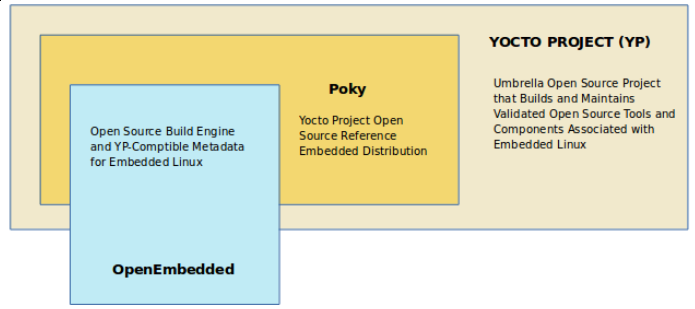
\includegraphics[width=0.5\textwidth]{yocto-project-block.png}
	\caption{Yocto Project structure, from \cite{yocto-manual}.} \label{fig:yocto-project-block}
\end{figure}

\subsection{Layer Model}

The Yocto development model defines a layered structure, as repositories that contain configurations and instructions for the OpenEmbedded build system to know what and how to build the system. The layer model allows to logically separate information in the build. If a layer needs to specify in another layer, a recipe defined in a BitBake append (\texttt{.bbapend}) file.

The common recommended workflow is based on a reference distribution (\textit{Poky}), which contains the OpenEmbedded build system and the set of metadata necessary to start building the IoT distribution.

\begin{figure}[htp]
	\centering
	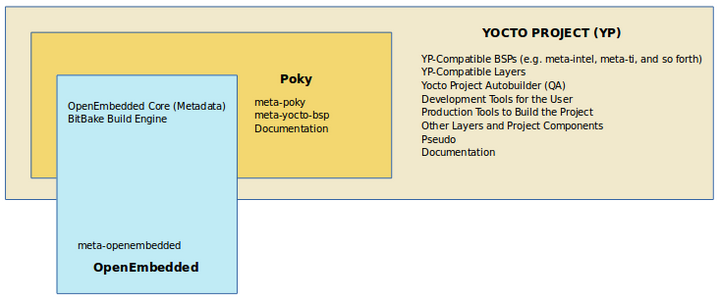
\includegraphics[width=0.5\textwidth]{yocto-poky.png}
	\caption{Content of a typical Poky repository, from \cite{yocto-manual}.} \label{fig:yocto-poky}
\end{figure}

\subsection{OpenEmbedded Build System Workflow}

The expected workflow can be represented in figure \ref{fig:yocto-workflow}, where the different actors are identified as well as the expected outputs. This process can be shortly summarized as follows:

\begin{enumerate}
	\item Specify architecture, policies, patches and configurations.
	\item Fetch and download of source codes.
	\item Sources extraction, patches applying and configuring and compiling the software.
	\item Software installing.
	\item Quality assurance and sanity checks for the entire build process.
	\item Binary package feed is used to create the final root file image.
	\item The build system generates the file system image and the Extensible SDK in parallel.
\end{enumerate}

\begin{figure}[htp]
	\centering
	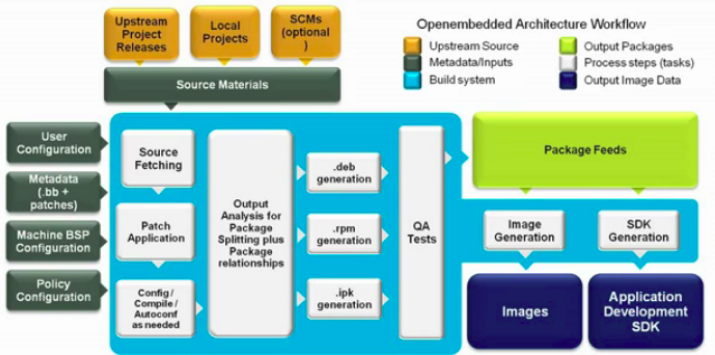
\includegraphics[width=0.5\textwidth]{yocto-workflow.png}
	\caption{Default Build System workflow, from \cite{yocto-manual}.} \label{fig:yocto-workflow}
\end{figure}

\section{Boot Up Sequence}

The embedded Linux built for this project requires a non-standard boot up flow, as the Znyq7 XC7Z010 chip has not enough MIO pins for the hardware that would allow the first boot read from an SD card reader. Therefore, a custom boot up sequence was needed. Additional, the board model was discovered to be a non-standar model (the typical model for the TE0726 includes 512MB of DDR3 RAM memory, whereas the model used is a 128 MB version), which created difficulties to find suitable documentation for this specific hardware configuration.

The process is detailed in the Appendix \ref{appen1}. As a general rule, the hardware definition for the PS needs to be done via a reference design project provided by the manufacturer using prepared scripts, as opposed to the usual Xilinx workflow where a user-defined board should provide a TCL preset file with the necessary configuration values for the IP Core.

Once the hardware has been correctly defined and exported, the Linux image build process needs to consider also the special configuration for the 128 MB memory capacity, which proved to be still a process with several iterations needed as the documentation and support is limited in terms of the manufacturer capabilities. The configuration also needs to define the boot process to the specific Zynq hardware configuration.

\subsection{Linux Boot}

\begin{figure}[htp]
	\centering
	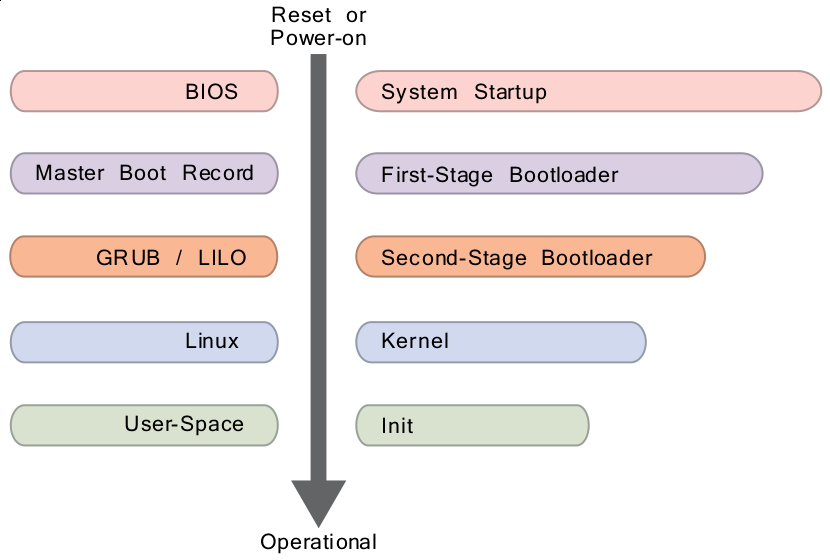
\includegraphics[width=0.5\textwidth]{linux-boot.png}
	\caption{Stages of a Linux boot process, from \cite{Crokett2014}.} \label{fig:linux-boot}
\end{figure}

\subsection{Zynq Boot}

\begin{enumerate}
	\item Power up of the board starts.
	\item The BOOT.BIN binary is read from flash memory through QSPI and run.
	\item From this binary, the First Stage Boot Loader is then loaded, which will configure the PS and PL, and then locate and load the u-boot into DDR memory.
	\item U-boot will initialize the hardware, and then unpack and load the linux kernel.
	\item Once the kernel is loaded into the high memory, specific hardware setup is run.
	\item When kernel is ready, the first user-space application (\textit{init}) can start.
\end{enumerate}

The specific process for the Zynqbery 726 board used in the project needs special considerations that are hardware-related. In general, the workflow provided by Xilinx needs to be slighltly modified, and use the board manufacturer documentation and scipts. This is due to the fact that the board uses specific hardware, and the documentation provided does not match. Once the image (and other relevant binary files) have been correctly build, special care needs to be taken to generate the BOOT.BIN file for the stage-0 boot process. More detailed instructions are provided in Appendix \ref{appen1}.

Once the image (and other relevant binary files) has been correctly build, special care needs to 

% TODO: Complete topic
